\documentclass[12pt]{article}
\usepackage{graphics}




\title{\textbf{Alpha Decay and Spontaneous Fission} \\
  \large Laboratory Exercise in SH2603}
\author{Lab assistant: Francesca Capel (capel@kth.se)}
\date{\today}
\begin{document}
\maketitle

\noindent Please come to the lab with a printed copy of these instructions.\\

\noindent
This laboratory exercise consists of three parts:
\begin{itemize}
\item A measurement of the range of alpha particles in air as a
  function of air pressure.
\item  Spectroscopy of an unknown alpha source.
\item  A measurement of the fragment energies from spontaneous fission
  of $^{252}\mbox{Cf}$. 


\end{itemize}

\noindent
{\bf Preparation:} In the laboratory a triple $\alpha$-source
containing the radioactive isotopes $^{244}\mbox{Cm}$, $^{241}\mbox{Am}$ 
and $^{239}\mbox{Pu}$ will be used for energy calibration of the
instrumentation. Calculate the $Q-$values of the alpha decays for these isotopes
using e.g. the Atomic Mass Table provided on the course homepage under "Reference material".
 Deduce the kinetic energies of the emitted
$\alpha$-particles from the $Q-$values.

\section*{Alpha Decay}
Alpha decay involves the spontaneous emission of an alpha particle
from an atomic nucleus. The alpha particle consists of two protons and
two neutrons and is the same species as the nucleus of a helium
($^{4}\mbox{He}$) atom.  These four nucleons have their origin in the
nucleus $X$ before the decay (the mother nucleus) and the nucleus is
therefore transformed into a nucleus $X'$ (the daughter nucleus) of
another basic element according to the relation:
\begin{equation}
^{A}_{Z}X_{N} \rightarrow ^{A-4}_{Z-2}X'_{N-2}+\alpha,
\end{equation}
where $\alpha$ is the alpha particle, $N$ is the number of neutrons,
$Z$ is the number of protons, and $A=N+Z$ is the mass number.

Several naturally occurring isotopes decay by alpha emission.
Figure~\ref{fig:radseries} shows the four \emph{radioactive series},
illustrating the chains of some heavy elements decaying by subsequent
alpha- and beta particle emission. The half-life of the single
isotopes in the chains varies over several orders of magnitude.
Radioactivity from these isotopes is often found when measuring
background radiation near or under ground, since ground minerals 
can contain uranium or thorium. These elements are also
often found in small quantities in house building materials. The inert
gas radon can escape the minerals, thereby making the air in an
insufficiently ventilated room radioactive.

\begin{figure}
\begin{center}
\resizebox{0.9\textwidth}{!}{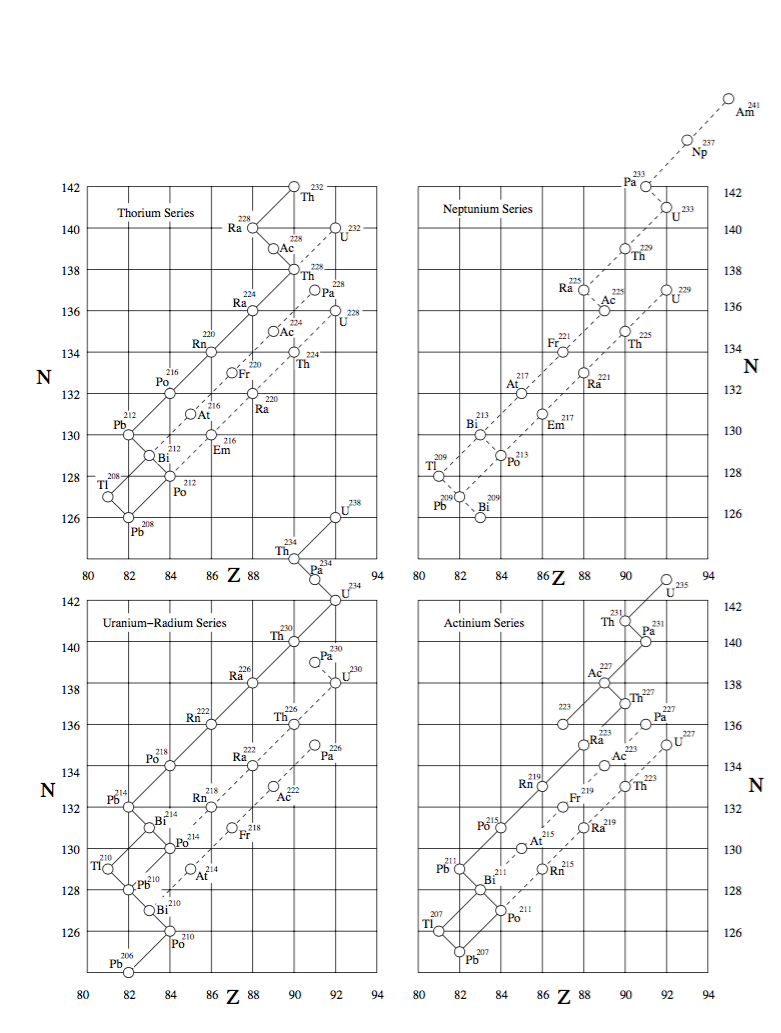
\includegraphics{radseries.png}}
\caption{The four radioactive decay series of the heavy elements. 
  Solid lines indicate naturally occurring decays, while dashed lines
  indicate decays from artificially produced radioactive isotopes.}
\label{fig:radseries}
\end{center}
\end{figure}

The alpha decay phenomenon has been utilised in a large number of
applications. Examples include smoke detectors, power sources in
unmanned spacecrafts and in cardiac pacemakers, and material analysis
methods, e.g. the Rutherford backscattering technique.

\section*{Spontaneous Fission}

For a limited number of heavy isotopes another decay mode, \emph{spontaneous
fission}, is strong enough to compete with alpha and beta decay. In
this process, the nucleus separates into two large parts. Usually, a
small number of neutrons are also released in the process.

If we compare the binding energy of a nucleus unstable to spontaneous
fission to the binding energies of some typical fission fragment
nuclei (e.g. see table in K.S. Krane, Appendix C), we immediately see
that an substantial amount of energy is released as a result of the
separation. This energy appears as kinetic energy of the two fission
fragments and the emitted neutrons.  The reason why the initial
nucleus lives for some time before fissioning is the existence of a
large energy barrier that must be overcome via tunnelling in order
for fission to occur.

\section*{The Interaction of Charged Particles in Matter}

Rutherford performed pioneering work in the early twentieth century by
studying the interaction of alpha particles with matter. This work, through
the experiments carefully performed by Geiger and Marsden, eventually
led to the discovery of the atomic nucleus.  The problem on how
charged particles interact with matter continued to be studied by
Niels Bohr and others, and later the theory was developed by Hans
Bethe and Felix Bloch. Thanks to these early efforts we have a good
understanding today about how charged particles are decelerated when
penetrating various materials.

When a charged particle at high velocity passes through a material it
will slow down and change direction due to interactions with
the surrounding atoms.  The 
first effect is mainly due
to inelastic scattering with atomic electrons in the material. The
electric field of the incoming particle can interact with electrons
several atomic distances from the particle trajectory and the
electrons are thereby excited into a higher atomic orbit or
completely detached from the atoms. If such a detached electron has
high enough energy, it can interact with other electrons and excite or
ionise the atoms. The electrons detached in such a subsequent
interaction are called secondary electrons, as opposed to the primary
electrons released by the interaction with the incoming charged
particle.

The process responsible for the change in direction for the
projectile is the elastic scattering against atomic nuclei
in the material. This is a rare process which has only a small
effect on the slowing down of heavy charged particles in matter.
Other less common processes, such as
nuclear reactions, can also occur depending on the energies 
and particles involved.

Since the deceleration of heavy charged particles in a material
typically involves a large number of interactions, it is meaningful
to introduce continuous quantities, such as the infinitesimal energy
loss per travelled length in the stopping material, also known as the \textbf{stopping power:} $\mathbf{\frac{dE}{dx}}$.

A theory for the energy loss of charged particles in matter was
developed by Bohr~\cite{Boh13b,Boh15} around the same time as he
developed his atomic model. The classical formula from this work
reads:
\begin{equation}
\label{eq:Bohr}
-\frac{\mbox{d}E}{\mbox{d}x}=\frac{4\pi z^2 e^4}{m_e v^2}N_e ln\frac{\gamma^2 m v^3}{ze^2 \hat{\nu}}
\end{equation}
This formulation gives reasonable results for alpha particles 
and heavier ions, but
does not work well for protons because of quantum effects. A proper
quantum mechanical approach was made by Bethe, Bloch and others
in the 1930s
resulting in the \emph{Bethe-Bloch formula}, the most well-known
expression for calculating the energy loss of charged particles in
matter:
\begin{equation}
\label{eq:Bethe-Bloch}
%-\frac{\mbox{d}E}{\mbox{d}x}=2\pi N_a r^2_e m_e c^2 \rho \frac{Z}{A}\,\frac{z^2}{\beta^2}
%\left[
%\mbox{ln} \left(
%\frac{2m_e \gamma^2 v^2 W_{\mbox{max}}}{I^2}
%\right)
%-2\beta^2
%\right],
-\frac{\mbox{d}E}{\mbox{d}x}=\left(
\frac{e^2}{4\pi\epsilon_0}
\right)^2
\frac{4\pi z^2 N_a Z \rho}{m_e c^2 \beta^2 A}
\left[
\mbox{ln} \left(
\frac{2m_e c^2 \beta^2}{I}
\right)
-ln(1-\beta^2)
-\beta^2
\right],
\end{equation}
where $v=\beta \cdot c$ is the velocity of the particle, $z$ is its
proton number, Z, A, and $\rho$ are the atomic number, atomic weight,
and mass density of the material. $N_a$ is Avogadro's number,
$m_e$ is the electron mass, and $I$ is the mean excitation energy
of the atomic electrons in the stopping material.

Modern calculations also include features like \emph{shell
corrections} and \emph{density corrections}~\cite{Leo93}.
Today, the energy loss for ions in several materials can
be calculated easily using existing computer software, e.g.
the SRIM programme~\cite{SRIM2003}. By dividing the stopping power by
the density of the material, the mass stopping power, $\frac{1}{\rho}$$\frac{dE}{dx}$,
is obtained. This is a useful quantity since the mass stopping power
varies less between different materials than the linear stopping power.

\section*{The Experimental Setup}
Since alpha particles and fission fragments have a limited range 
in air at normal pressure, we have to remove the air between 
the source and the detector. Two different vacuum
chambers are used in the exercise. A schematic picture of the setup
is drawn in figure~\ref{fig:setup1}.  A mechanism for changing
radioactive sources is mounted in the large chamber. In this way, we
can choose between any of three different sources (and one empty
position) without breaking the vacuum.  In the small vacuum chamber
(located in a NIM module together with the electronics) we can control
the air pressure by adjusting a valve. You may open the small vacuum
chamber (when it is at atmospheric pressure) and inspect the $\alpha$ source
and the Si surface barrier detector. Be careful not to touch the surface
of the $\alpha$ source! In both vacuum chambers we use the same
type of surface barrier semiconductor (Si) detector. The energy signals from the Si
detector are amplified and shaped by the preamplifier and main amplifier modules
and subsequently digitised and stored by a multi-channel analyser
(MCA) card residing in a PC .  The \emph{TUKAN} software displays the energy data on
the computer screen and can be used to analyse the spectrum.

\begin{figure}
\begin{center}
\resizebox{\textwidth}{!}{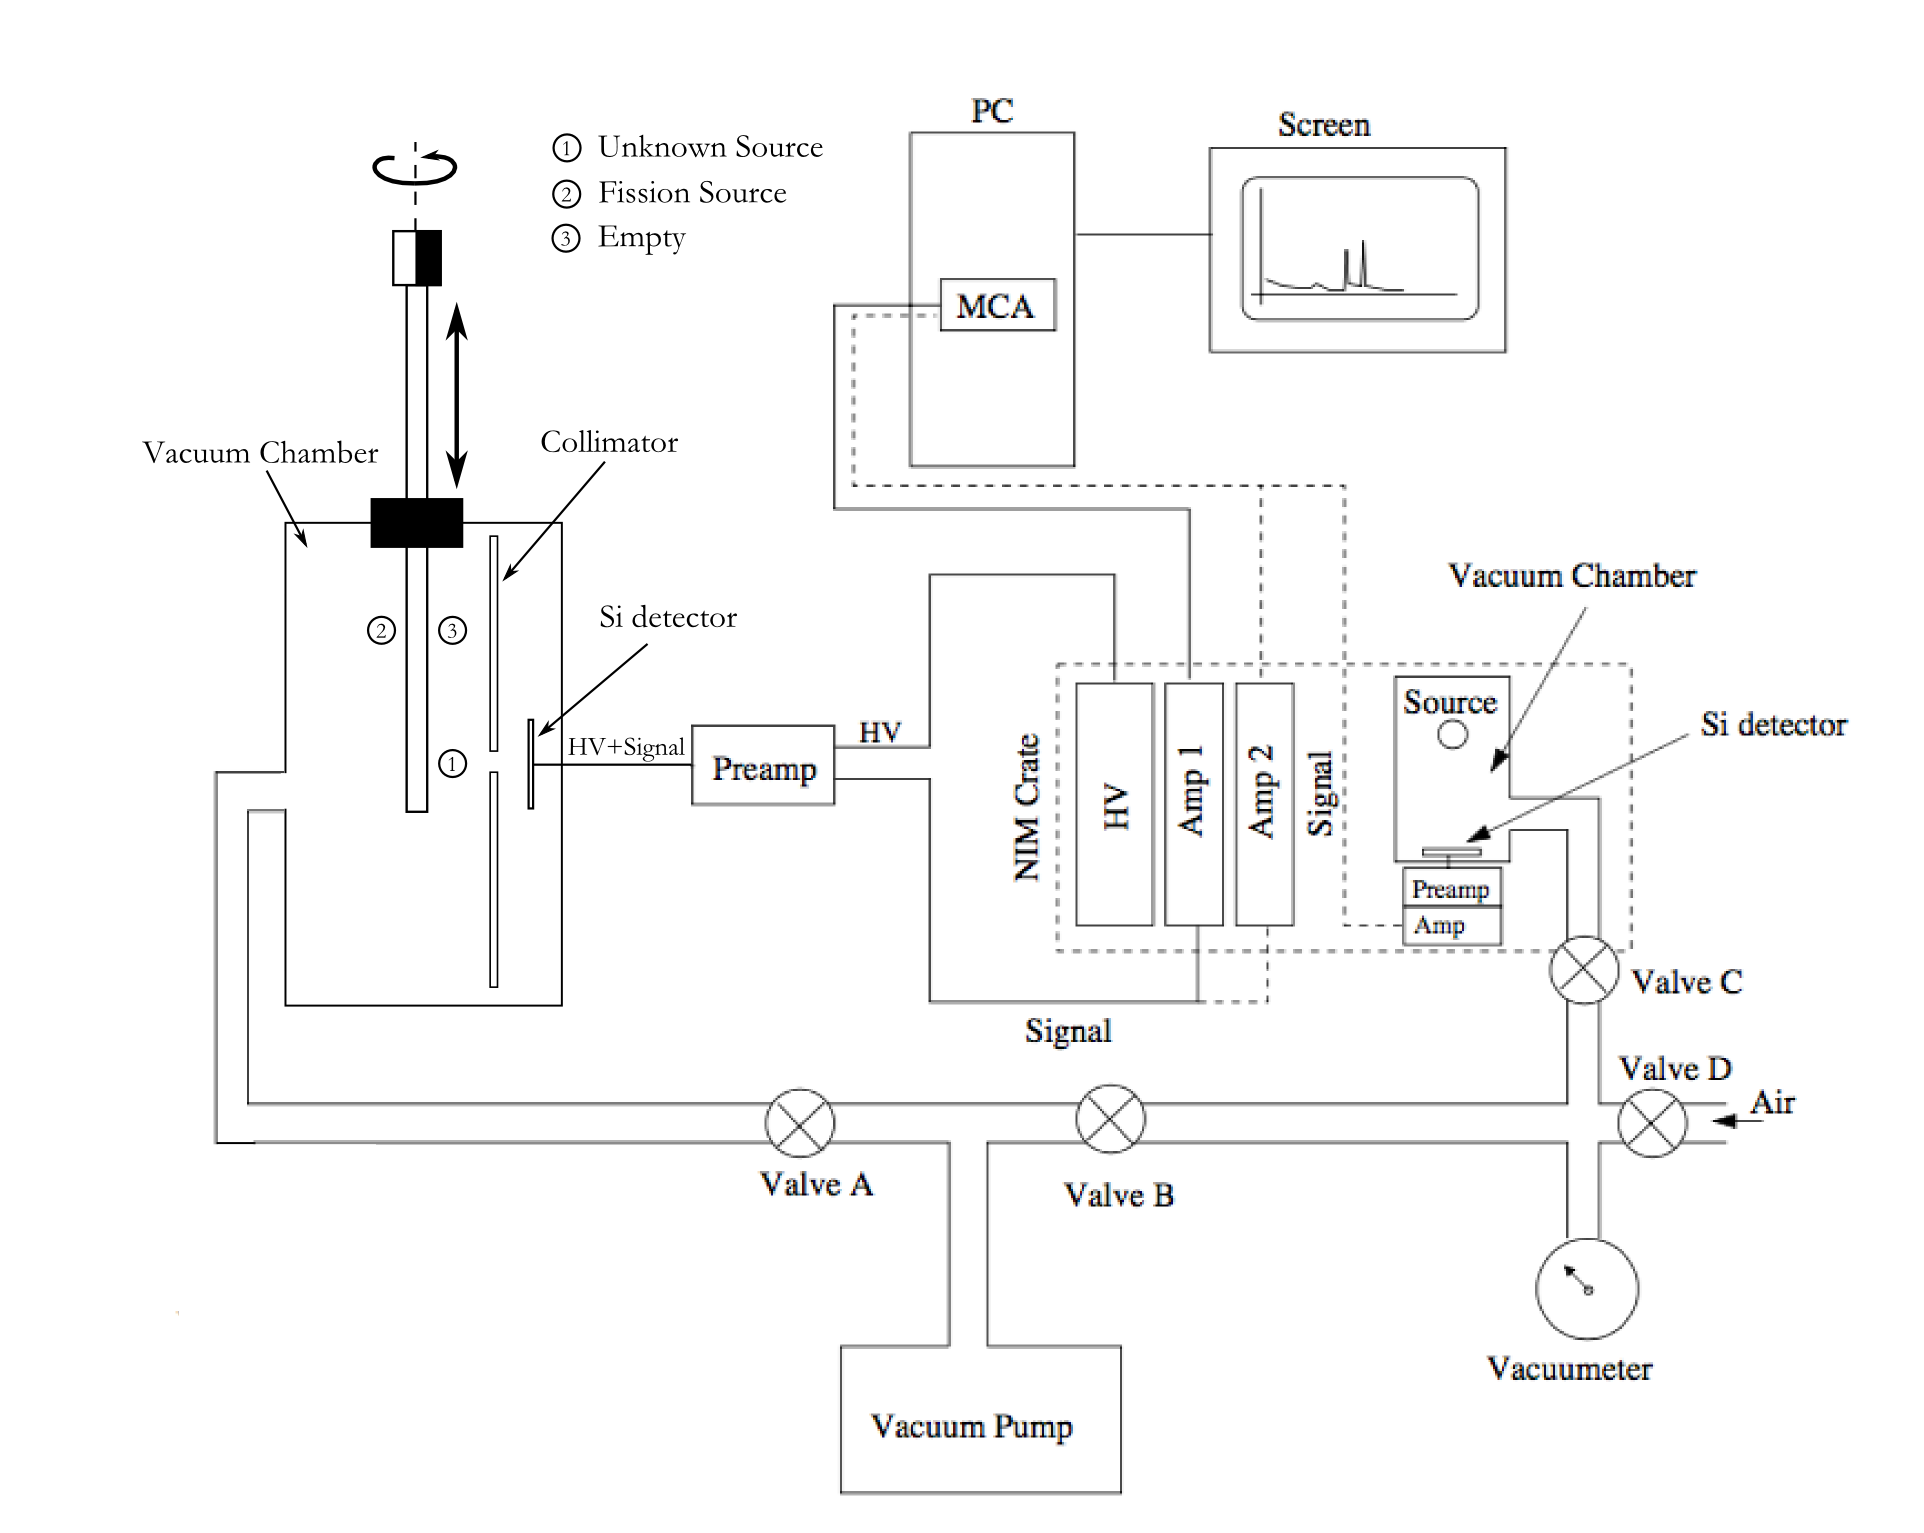
\includegraphics{setup2.png}}
\caption{A schematic view of the two vacuum chambers and the electronics
  for energy measurements of alpha particles and fission fragments. A
  surface barrier silicon detector (one in each chamber) is used to
  detect the energy of the incoming particles.  Two different
  radioactive sources are mounted on a manipulator rod in the large
  vacuum chamber. A third position is used when not measuring.  By
  pulling/pushing or rotating the rod 180$^\circ$, the source of
  interest is put in front of the collimator and the detector is then
  shielded from the other one. The rod should be placed in
  position \#3 when the measurements are finished, so that the
  detector is not irradiated unnecessarily.  The venting valve (D) in
  the picture is used to control the pressure in the small vacuum
  chamber by letting in small amounts of air at a time. A
  multi-channel analyser (MCA) card together with \emph{TUKAN} software
  in the PC is used to collect the data. The energy spectrum is 
  displayed on the computer screen. The two main amplifiers \#1 and \#2 
  can be set at a high and a low gain in order to accomodate 
  the different energy ranges for $\alpha$ particles and fission fragments, respectively.}
\label{fig:setup1}
\end{center}
\end{figure}

\section*{Questions to answer before the laboratory exercise}

Find the answer to the following questions and discuss
them with the assistant before starting the measurements.

\begin{itemize}
  
\item How can the physical mechanism behind alpha decay be described
  in simple terms?

\item What can we say in general about the efficiency and size of a typical
alpha particle detector?

\item Will the range (in for example silicon)
of a typical fission fragment be larger or smaller than the
range of an alpha particle at a typical decay energy?

\item Explain why alpha decay is sometimes accompanied by
  gamma emission.

\end{itemize}

\section*{Measurements and Safety}

This exercise involves open alpha sources which are to be handled only by the
assistant due to risk of contamination.\\

\noindent No food or drink is allowed in the lab.\\

\noindent Wash your hands when leaving the lab.\\

\noindent Before starting the measurements, let the laboratory assistant explain
the proper handling of the vacuum system.  In case of incorrect
use, oil from the vacuum pump can pass into the vacuum chamber and damage the
Si detector. Follow the lists of points below to perform the measurements.

\section{Determination of the Range of Alpha Particles in Air}

Before we do the actual measurements we must calibrate the detector so that
we have an accurate measurement of the particle energy.

\subsection{Calibration}

The triple alpha source ($^{244}\mbox{Cm}$, $^{241}\mbox{Am}$ 
and $^{239}\mbox{Pu}$) with
known alpha energies is used to obtain a good energy calibration.

\begin{itemize}
\item Place the source inside the small vacuum chamber.
\item Without touching the source, measure the distance from the source
 to the Si detector.
\item Aquire a spectrum using the TUKAN software. Explain the details of the spectrum. 
Can one alpha decay give rise to more than one peak? Look in the \emph{Table of Isotopes} 
(or NUDAT2) and discuss with the assistant.
\item Use the deduced energies of the main alpha peaks to calibrate the spectrum.
\end{itemize}

\subsection{Measurements}

\begin{itemize}
  
\item Think of how you can determine the range of the alpha particles
  in air at atmospheric pressure using the equipment at hand.
  
\item Meausure the alpha particle energies as a function of pressure. Use the vacuum valve to control the air
  pressure in the chamber. Measure at about ten different pressure values. Plot the results.

\item Record also the energy resolution as a function of pressure. Can you explain the observed effect?

\item Deduce the range of the alpha particles in air at 1 atm.

\item Produce a $\frac{dE}{dx}$ curve for alpha particles in air.
\end{itemize}


\section{Unknown Source}
The source in position \#1 in the large vacuum chamber is an
unknown source that contains naturally occurring radioactive isotopes.
\begin{itemize}
\item Measure the energies from the unknown alpha source.
\item Compare with the decays of the radioactive series, see 
figure~\ref{fig:radseries}. Use the \emph{Table of Isotopes}. 
What element/elements is/are involved? What material is the unknown 
source made of?
\item Can we say anything about the age of the source?
\end{itemize}

\section{Spontaneous Fission}
The radioactive source placed in position \#2 in the large
vacuum chamber is $^{252}\mbox{Cf}$. This nuclide is unstable against
alpha decay as well as spontaneous fission.
\begin{itemize}
\item Collect data to obtain a new energy spectrum. Adjust the amplifier 
to see details in different energy regions. Identify both fission
fragment bumps and the alpha peaks. Determine the alpha energies.
\item What are the approximate energies for the fission fragment
  distributions?  Can we rely on these energies with the current
  calibration?  Discuss with the assistant.
\item What can we say about the mass distribution of the two fission
  fragments? Which fission fragment bump belongs to which fission
  fragment mass distribution (large/small masses)?
\item Finally determine the branching ratio between alpha decay and
  spontaneous fission in $^{252}\mbox{Cf}$. Be sure to include an associated 
  statistical error with your result. 
\end{itemize}


\section*{Report}
The students should write a report after the laboratory exercise to be handed
in to the laboratory assistant two weeks after the day of the laboration.


\bibliography{alphalab}
\bibliographystyle{unsrt}

\end{document}
